\documentclass[../rapport.tex]{subfiles}
\graphicspath{{\subfix{ressources/photos_diagrammes/}}}


\begin{document}
	
	\begin{figure}[h]
		\centering 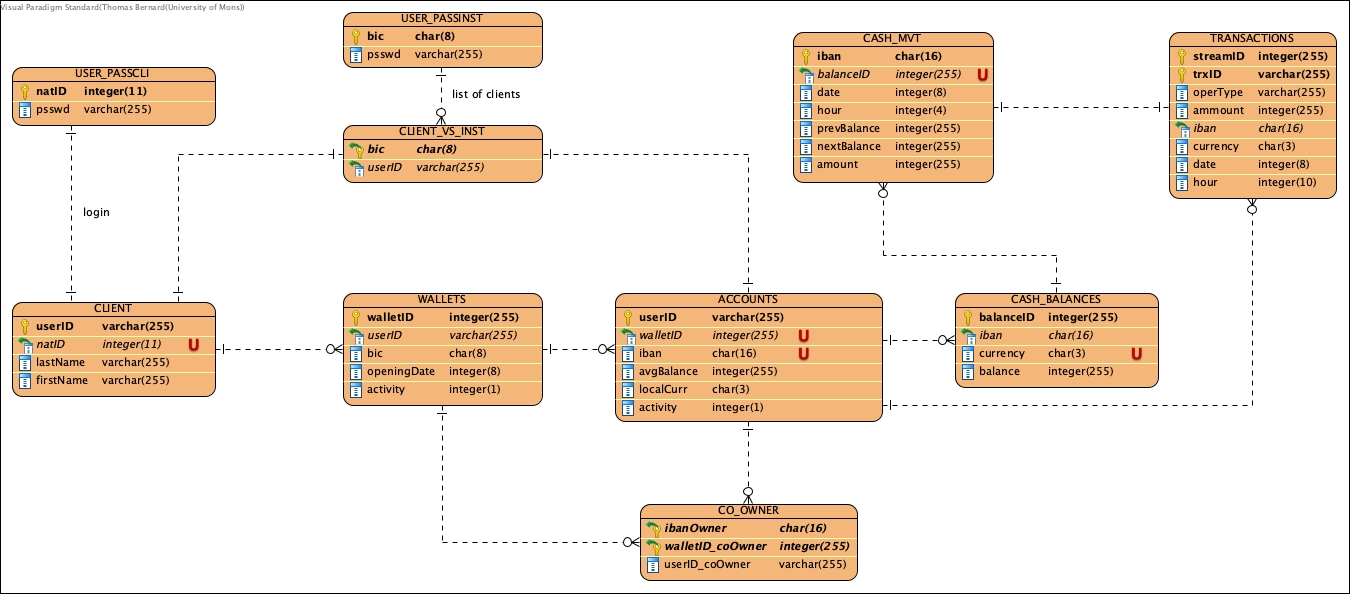
\includegraphics[scale=0.3]{ressources/photos_diagrammes/erd.jpg}
		\caption{Diagramme d'entité-relation de l'application.}
	\end{figure}
	
	\paragraph{Tables utilisateurs :}
	Pour notre base de données nous avons essayé de séparer au mieux les tables afin que celles-ci restent simples de compréhension et faciles d'accès. Nous avons une table \textbf{USER\_PASSCLI} qui sert de table d'authentification. Elle contient le mot de passe \textbf{psswd} ainsi que le numéro de registre national de l'utilisateur \textbf{natID} si les deux correspondent alors on peut accéder à la table \textbf{CLIENT} qui contient quant à les informations personnelles du client ainsi que son nom d'utilisateur \textbf{userID}.
	
	\paragraph{Tables des institutions :} Afin que les insitutions n'aient pas accès à la notion de portfeuilles nous avons introduit 2 tables qui leurs sont propres et qui permettent de faire le lien entre les clients de la table \textbf{CLIENT} et leurs produits financiers de la table \textbf{ACCOUNTS}.
	
	\medskip
	
	La table \textbf{USER\_PASSINST} est à l'image de la table 
	\textbf{USER\_PASSCLI} une table d'authentification pour les institutions à l'aide de leur identifiant \textbf{bic}. 
	
	\medskip
	
	La table \textbf{CLIENT\_VS\_INST} associe chaque client et institution si pour un \textbf{userID} il possède au moins un produit financier dans l'insitution. Lorsqu'un \textit{wallet} est créé le \textbf{userID} du client ainsi que le \textbf{bic} de l'institution dans lequel il est créé sont ajoutés à la table ce qui permet ainsi à l'instution de récupérer la liste de ses clients assez aisément à l'aide de cette table. De plus elle peut ensuite se servir du \textbf{userID} afin de récupérer la liste des produits du client (table \textbf{ACCOUNTS} ainsi que ses informations personnelles (table \textbf{CLIENT}).
	
	\bigskip

	\paragraph{Autres tables}

	La table \textbf{WALLETS} est la table qui contient tous les portefeuilles de 
	clients. Lorsqu'un portfeuille est créé en plus d'ajouter le portfeuille dans 
	la table \textbf{WALLETS} on ajoute également le userID ainsi que le bic de 
	l'institution dans laquelle le portfeuille a été créé dans la table
	\textbf{CLIENT\_VS\_INST} afin que l'institution qui n'a pas accès à la table 
	\textbf{WALLETS} puisse tout de même savoir quels clients sont clients de son
	institution et n'ait accès qu'à ceux-ci dans la table.
		
	\medskip

	Cette table possède une Primary Key qui est le walletID et qui attribue à chaque
	portfeuille d'un client un numéro de suite qui unique. Ce numéro permettra entre
	autres dans l'application client de récupérer tous les produits d'un 
	portefeuille. Le userID références la table \textbf{CLIENT} afin d'avoir ses
	informations dans son portfeuille.
	\bigskip

	La table \textbf{ACCOUNTS} contient les produits financiers de type Comptes 
	bancaires. Chaque compte est identifié de manière unique grâce à son iban.
	Cette table référence la table \textbf{WALLETS} grâce au walletID qui permet 
	de n'avoir que les produits d'un portefeuille. 

	\bigskip

	La table \textbf{CO\_OWNERS} est une table contenant la liste de tous les 
			co-titulaires. Dans celle-ci on retrouve l'ibanOwner qui référence vers
			la table \textbf{ACCOUNTS} et permet au posseseur du compte de savoir
			qui est co-titulaire et de le gérer. Cette table possède également le
			walletID\_coOwner qui référence vers la table \textbf{WALLETS} et qui 
			permet au co-titulaire de récupérer également les comptes qui ne sont
			pas en sa possession. Enfin il y a aussi le userID\_coOwner qui permet 
			aux institutions de voir les co-titulaires des comptes.

		\bigskip 
		
	La table \textbf{CASH\_BALANCES} contient les différents soldes d'un compte
	bancaire. En effet un compte dans l'application de base n'a qu'un solde EURO
	mais pour des soucis de simplicité de création de la base de données la 
	possibilités d'avoir des soldes dans d'autres devises a déjà été ajoutée.

	\medskip

	La clé primaire de cette table est le balanceID qui est un numéro de suite 
	unique permetttant d'identifier chaque solde d'une devise d'un compte. 
	La currency pour une balanceID est unique dans cette table car un compte
	ne peut pas posséder plusieurs soldes dans la même devise. La table référence
	la table \textbf{ACCOUNTS} à l'aide de l'iban du compte afin d'obtenir tous les
	soldes d'un compte.

	\bigskip

	La table \textbf{TRANSACTIONS} est une liste de transactions à effectuer. Une 
	transaction est composée de 2 flux ( l'ascendant et le descendant ) Mais dans 
	ce cas, un élément de la table ne reprend qu'un seul des 2 flux car les 2 
	flux ne sont pas liés au même compte bancaire. C'est pourquoi il ya un colonne 
	trxID qui est un numéro de suite de transaction. Ce numéro de suite est attribué
	aux 2 flux (streamID) d'une transaction et permet de vérifier que les 2 flux 
	ont bien été exécutés avant d'appliquer les changements aux soldes. 

	\medskip

	Cette table référence la table \textbf{ACCOUNTS} à l'aide de l'iban d'un flux 
	car c'est à partir d'un compte que l'on effectue une transaction. Ce même iban
	référence également la table \textbf{CASH\_MVT}.

	\bigskip

	La table \textbf{CASH\_MVT} est la table d'historique des transactions. Dans 
	cette table ne se trouve que les mouvements qui ont été réalisés avec succès.
	Cette table est liée à la table transaction par l'iban afin d'ajouter un 
	élément dès qu'une transaction est complétée. 

	\medskip

	C'est cette table qui se charge de mettre à jour les les soldes. Si un élément 
	est ajouté à la table c'est que la transaction a bien eu lieu. Donc, grâce au 
	balanceID qui référence la table \textbf{CASH\_BALANCES} et au ammount on peut
	effectuer la mise à jour du solde du compte.

\end{document}
